%
% Modified by Megan Patnott
% Last Change: Jan 18, 2013
%
%%%%%%%%%%%%%%%%%%%%%%%%%%%%%%%%%%%%%%%%%%%%%%%%%%%%%%%%%%%%%%%%%%%%%%%%
%
% Modified version of the sample_ndthesis.tex
% by Sameer Vijay
% Last Change: Wed Jul 27 2005 14:00 CEST
%
%%%%%%%%%%%%%%%%%%%%%%%%%%%%%%%%%%%%%%%%%%%%%%%%%%%%%%%%%%%%%%%%%%%%%%%%
%
% Sample Notre Dame Thesis/Dissertation
% Using Donald Peterson's ndthesis classfile
%
% Written by Jeff Squyres and Don Peterson
%
% Provided by the Information Technology Committee of
%   the Graduate Student Union
%   http://www.gsu.nd.edu/
%
% Nothing in this document is serious except the format.  :-)
%
%%%%%%%%%%%%%%%%%%%%%%%%%%%%%%%%%%%%%%%%%%%%%%%%%%%%%%%%%%%%%%%%%%%%%%%%
% This is *not* a substitute for the documentation, which is included
% as a pdf file in the standard distribution, and can be obatined from
% the dtx file in the advanced distribution.
%%%%%%%%%%%%%%%%%%%%%%%%%%%%%%%%%%%%%%%%%%%%%%%%%%%%%%%%%%%%%%%%%%%%%%%%
%
% You should *also* have a ND formatting guide to ensure that you have
% all the relevant parts, put the captions in the right place, etc.
% Just because you have this wonderful style classfile doesn't mean
% that it removes *all* the formatting onus from you.  :-)
% Although be warned that the Graduate School has been known to let
% their official formatting guide get out of date. When in doubt,
% the Microsoft Word example seemed to be the only thing kept
% consistently up-to-date in 2013, and is probably the safest thing
% to consult.
%
% You should break all of this stuff up into separate files
% (at the very least, one chapter per file) and use the \include
% command, as has been done here for chapters 1 and 2 and the appendix.
% There is also an \input command, but \include is more commonly used to
% import chapters in books and dissertations. For the differences between these
% two commands, see, e.g., 
% http://web.science.mq.edu.au/~rdale/resources/writingnotes/latexstruct.html
% or http://tex.stackexchange.com/questions/246/when-should-i-use-input-vs-include.
%
% If you compile from the command line, note that you should also have 
% a good Makefile; one that invokes LaTeX as many times as necessary 
% (up to 4) and bibtex if necessary.
%
% If you use an editor that allows you to compile from within the
% program, note that you will need to compile up to four times. Also,
% we recommend that you use pdflatex (sometimes displayed as
% LaTeX => PDF) to compile directly to pdf.
%
% If you have any suggestions, comments, questions, please send e-mail
% to: dteditor@nd.edu
%
%%%%%%%%%%%%%%%%%%%%%%%%%%%%%%%%%%%%%%%%%%%%%%%%%%%%%%%%%%%%%%%%%%%%%%%%

\documentclass[final,numrefs,sort&compress,twoadvisors]{nddiss2e}
% One of the options draft, review, final must be chosen.
% One of the options textrefs or numrefs should be chosen
% to specify if you want numerical or ``author-date''
% style citations.
% Other available options are:
% 10pt/11pt/12pt (available with draft only)
% twoadvisors
% noinfo (should be used when you compile the final time
%         for formal submission)
% sort (sorts multiple citations in the order that they're
%       listed in the bibliography)
% compress (compresses numerical citations, e.g. [1,2,3]
%           becomes [1-3]; has no effect when used with
%           the textrefs option)
% sort&compress (sorts and compresses numerical citations;
%           is identical to sort when used with textrefs)

\begin{document}

\frontmatter % All the items before the first chapter go in ``frontmatter''

% Titles may be 1-4 lines long. If your title is longer than 4 lines,
% the class file may have difficulty formatting the title page.
% Line-breaks in the title have to be protected with `\protect`.
\title{Gnus and you \protect\\ a Brief \protect\\ on all and
Everything \protect\\ About Gnus in our Society}
\author{Gerald G. Gnastich}
\work{Dissertation} % or \work{Thesis}
%\degaward{Doctor of Philosophy} % or 
\degaward{Master of Science \\ in \\ Subject}
\advisor{Gary Greenfield}
\secondadvisor{Gordon Gray} % if you have two advisers are using the option twoadvisors
\department{Gnulogy}

\maketitle
%%%%%%%%%%%%%%%%%%%%%%%%%%%%%%%%%%%%%%%%%%%%%%%%%%%%%%%%%%%%%%%%%%%%%%%%
%
% Front stuff
%
%%%%%%%%%%%%%%%%%%%%%%%%%%%%%%%%%%%%%%%%%%%%%%%%%%%%%%%%%%%%%%%%%%%%%%%%

% You must either set the copyright information or put your work in the public domain.
\copyrightholder{Garry Greene} % See template or documentation for
\copyrightyear{2005}           % other copyright options.
\copyrightlicense{CC-BY-4.0}
\makecopyright

% An abstract is optional for a mster's thesis, and required for a doctoral dissertation.
\begin{abstract}
  Please note that the full \LaTeX\ source code (and an associated
  \texttt{Makefile}) is available from the University of Notre Dame
  Graduate Student Union web site.  The Information Technology
  Committee page\footnote{\url{http://www.gsu.nd.edu/}}
  has all the necessary files in download-able form.  This particular
  dissertation was developed under Unix, but is also be usable
  under Windows with the appropriate \LaTeX\ setup and was modified
	on a Windows system in 2012-2013. It should also work with on Mac.
  
  While the source code for this document provides an excellent
  example for how to use the \nddiss\ \LaTeX\ class to write a
  Notre Dame thesis, it is \emph{not} a substitution for the
  documentation of the \nddiss\ \LaTeX\ class (also available on
  the ND GSU web site).

  In this thesis, I will tell all that I know about Gnus.  Gnus are
  wonderful little creatures that inhabit the center of the earth and
  give us wonderful and plentiful trees, dirt, and other
  earthly-things.
  
  In short, we should love and cherish the Gnus.  They can be very
  friendly, and are often mistaken for squirrels on the University of
  Notre Dame campus.  Feed them whenever possible.  If they get caught
  in trash cans, tip them over so that they can get out.

  This abstract is going to continue on, including a few formulas,
  just for the sake of spilling over on to two pages so that we can
  see the author's name in the top right corner:
  
	\begin{align*}
    a^2 + b^2 &= c^2 \\
    E &= mc^2 \\
    \frac{e}{m} &= c^2 \\
    a^2 + b^2 &=\frac{e}{m}
  \end{align*}

  These equations, by themselves mean nothing.  But to the common Gnu,
  they define a whole way of living.  While intricate mathematical
  implications certainly do not infiltrate the majority of humans'
  lives, every Gnu, from birth, is imbued with a sense of mathematical
  certainty and guidance.  All Gnus, great and small, feel at one with
  mathematics.  The cute furry bit is just a scam for their
  calculating minds.
\end{abstract}

% A dedication is optional.
\renewcommand{\dedicationname}{NEW DEDICATION NAME}

\begin{dedication}
  To George, my favorite Gnu
\end{dedication}

% These are required, and must be in this order.
\tableofcontents
\listoffigures
\listoftables

% A preface is optional.
\begin{preface}
  I would like to preface this work with all the wonderful things that
  Gnus have brought to our society: trees, dirt, flowers, grass,
  lakes, and other earthly-things.  We should not forget them in our
  daily lives.

  Additionally, we should offer them food for all their hard work.  In
  fact, Gnus work so hard that they sleep for the colder half of
  the year.  As such, they tend to grow a little rotund.  Humans
  should not fault them for this, as it is necessary for their
  survival.  Indeed, many humans grow rotund on their on accord!
\end{preface}

% It's hard to tell from the information available from the Graduate
% School in Spring 2013 whether or not an acknowledgements section is optional.
\begin{acknowledge}
  I would like to acknowledge all the loving Gnus at Notre Dame.
  Particularly the one that comes to the window in the Hayes Healy
  building.  He (she?) has given me much inspiration, love, and dirt.
  I would also like to thank my advisor, Dr.\ Gary Greenfield, with
  whom this work would not have been possible.

  Finally, I would like to thank the U.S.\ Government, Department of
  Gnus, for their generous grant, number GNU3042920920.3, which
  allowed me to pursue my work.
\end{acknowledge}

% A symbols section is optional.
\begin{symbols}
  \sym{\mathcal{F}}{sighting frequency of Gnus about campus}
  \sym{p}{student population}
  \sym{f}{type of food available}
  \sym{d}{day of week}
  \sym{c}{speed of light}
  \sym{m}{mass}
  \sym{e}{elementary charge}
  \sym{a,b}{miscellaneous constants}  
  \sym{E}{energy}  
\end{symbols}

\mainmatter
% Place the text body here.
%\include{chapter-one}
%Begin each chapter with \chapter{Title}. Both the thesis title and
%chapter titles should match in style.

%
% An unnumbered chapter (features)
%
\unnumchapter{Features of Formatting in This Example File}
% The \unnumchapter command allows you to include an unnumbered chapter as part of
% the main text before Chapter 1. It will appear in your table of contents, and you
% should have at most one such chapter (although nothing in the class file will
% prevent you from creating more).

% The usual \cite{} command is also available, and should work as expected.
This \verb+chapter+ has been added to the original sample file to highlight the
various features with the formatting that conforms to the Graduate school
guidelines --- whether obtained due to the use of \nddiss\/ class file or just
plain good practice.
\begin{itemize}
\item An important note on line-breaks via \verb+\\+ in titles: the
  titles of the thesis as well as chapters and table captions use
  \verb+\MakeTextUppercase{}+ from the \verb+textcase+ package.  Due
  to the nature of the \verb+center+ environment, any line-breaks
  introduced in titles and captions should be protected, as in
  \verb+\protect\\+.
  To preserve the case in titles and captions, use, e.g.,
  \verb+\NoCaseChange{Gnus}+.
\item In the \emph{dedication}, the title name has been modified. So, you know
how to and that it can be done.
\item The entries in the \emph{List of figures} and \emph{List of Tables} are
single-spaced themselves but are double-spaced from the other.
\item The table captions are not in all CAPS as well for the reason mentioned
above.
\item Appropriate space is left between the \verb+Table xx+ and its
corresponding caption (which is double-spaced itself) as in table \ref{tbl:bogus1}.
\item Tables look much better without the vertical lines (good practice).
\item There is double-spacing between the table entries but single-spacing
within the entry.
\item The chapter (see Chapter \ref{chap:golfing}) or section titles are
double-spaced as mentioned in the guidelines.
\item There is a \verb+subsubsection+ present (eg. section \ref{sec:data}) and
is properly formatted in the TOC.
\item Sections deeper than \verb+subsubsection+ should not appear in the TOC.
\item Table \ref{tbl:defs} is an example of the use of \textsf{landscape}
environment in which a normal table is formatted in a \emph{landscape} mode.
\item The \textsf{longtable} environment is used in Tables \ref{tbl:votes} and
\ref{tbl:rotated-rankings}, in normal and \verb+landscape+ mode, respectively. The
table captions are formatted properly in both cases.
\item In the table \ref{tbl:votes}, the \verb+footnote+ in the table header 
does not appear at all. This is not an error of the \nddiss\/ class but of the
\textsf{longtable} package.
\item An example of citing a website is shown in the bibliography (see
\citep{gairley2000}) which is formatted using the \verb+nddiss2e.bst+
citation style file.
\item A bit of information on the \nddiss\/ class file and the typesetting program
used is included in a box on the last page of the thesis.
\item Footnotes should space properly.
\item Items in \verb+itemize+, \verb+enumerate+, and \verb+description+ environment
should automatically single-space within an item, but double space between items.
\end{itemize}

%
% Chapter 1
%

%
% Modified by Megan Patnott
% Last Change: Jan 18, 2013
%
%%%%%%%%%%%%%%%%%%%%%%%%%%%%%%%%%%%%%%%%%%%%%%%%%%%%%%%%%%%%%%%%%%%%%%%%
%
% Modified by Sameer Vijay
% Last Change: Tue Jul 26 2005 13:00 CEST
%
%%%%%%%%%%%%%%%%%%%%%%%%%%%%%%%%%%%%%%%%%%%%%%%%%%%%%%%%%%%%%%%%%%%%%%%%
%
% Sample Notre Dame Thesis/Dissertation
% Using Donald Peterson's ndthesis classfile
%
% Written by Jeff Squyres and Don Peterson
%
% Provided by the Information Technology Committee of
%   the Graduate Student Union
%   http://www.gsu.nd.edu/
%
% Nothing in this document is serious except the format.  :-)
%
% If you have any suggestions, comments, questions, please send e-mail
% to: ndthesis@gsu.nd.edu
%
%%%%%%%%%%%%%%%%%%%%%%%%%%%%%%%%%%%%%%%%%%%%%%%%%%%%%%%%%%%%%%%%%%%%%%%%


%
% Chapter 1
%

\chapter{Introduction}

\section{Overview}

This is an overview of the introduction.  In here, I will use many
many buzzwords and other legalistic-types of terms, mostly beginning on
the expounding of the holistic and synergistic energy that Gnus bring
to our organizations.

\subsection{Background}

In preparation for reading this dissertation, I would highly recommend
reading some of the other material available on
Gnus~\citep{gnus98:_gerry_ganst,greenfield96:_gettin_know_gnu}.  They
are very well written and will give you a fuller understanding of
Gnus.

Gnus are frequently mistakes for squirrels.  They are not squirrels.
They are Gnus.  Don't call them squirrels, either (unless you have
food in your hand); they tend to get a bit upset.\footnote{This is
  frequently mistaken for the chattering and scampering away.  Gnus
  are actually quite polite; they will leave if they have nothing nice
  to say, for fear of saying something offensive.}  If you have food
in your hand, they tend to ignore this insult and accept your food as
a peace offering.\footnote{Sometimes they'll follow you if you continue
to refuse to feed them.}

\subsection{Foreground}

Table~\ref{tbl:bogus1} shows some feeding frequencies for where Gnus
like to eat around the Notre Dame campus.  Gnus have work weeks, just
like humans do, hence the much lower frequencies on weekends.  This
can lead us to conclude that Gnu weekend shifts are much smaller than
the normal work-week shifts.  In fact, we can attempt to parametrize the
sighting frequency, $\mathcal{F}$, by the student population, type of food, and
day of the week as:
\begin{equation}
  \mathcal{F} = \mathcal{F}(p,f,d).
\end{equation}
Table~\ref{tbl:bogus2} shows what they
typically like to eat.

\begin{table}[tpb]
  \begin{center}
    \caption{Where \NoCaseChange{Gnus} Like to eat \label{tbl:bogus1}}
    \begin{tabularx}{0.85\textwidth}{lrrrrrrr} \toprule
      \multicolumn{1}{c}{Location} & Sun & Mon & Tue & Wed & Thu & Fri & Sat \\ \midrule
      Front of Dome & 1 & 5 & 6 & 5 & 4 & 5 & 1 \\
      Stonehenge & 2 & 9 & 10 & 12 & 9 & 14 & 2 \\
      The Rock & 1 & 3 & 4 & 3 & 4 & 3 & 0 \\
      The ACC & 3 & 4 & 5 & 5 & 5 & 4 & 1 \\
      Dining Halls & 5 & 14 & 12 & 13 & 14 & 12 & 3 \\
      Hesburgh Library & 2 & 3 & 5 & 2 & 3 & 4 & 2 \\ \bottomrule
    \end{tabularx}
  \end{center}
\end{table}

\begin{table}[tpb]
  \setlength{\capwidth}{0.7\textwidth}
  \begin{center}
    \caption{What \NoCaseChange{Gnus} like to eat on the Notre Dame Campus, Listed
      by Average Number of Sightings per Weekday
    \label{tbl:bogus2}
}
    \begin{tabular}{lrrrrrrr} \toprule
      \multicolumn{1}{c}{Food} & Sun & Mon & Tue & Wed & Thu & Fri & Sat \\ \midrule
      Twinkies & 1 & 5 & 6 & 5 & 4 & 5 & 1 \\
      Ding Dongs & 2 & 9 & 10 & 12 & 9 & 14 & 2 \\
      Carrots & 1 & 3 & 4 & 3 & 4 & 3 & 0 \\
      Lettuce & 3 & 4 & 5 & 5 & 5 & 4 & 1 \\
      Twizlers & 5 & 14 & 12 & 13 & 14 & 12 & 3 \\
      Jawbreakers & 2 & 3 & 5 & 2 & 3 & 4 & 2 \\ \bottomrule
    \end{tabular}
  \end{center}
\end{table}

Figure~\ref{fig:bogus3} shows a nice graph of location distributions
by day of week.  I have no real reason for including it except to show
that figures work as well.  Did I mention that Gnus are really cool?

\begin{figure}[tpb]
  \begin{center}
    \centerline{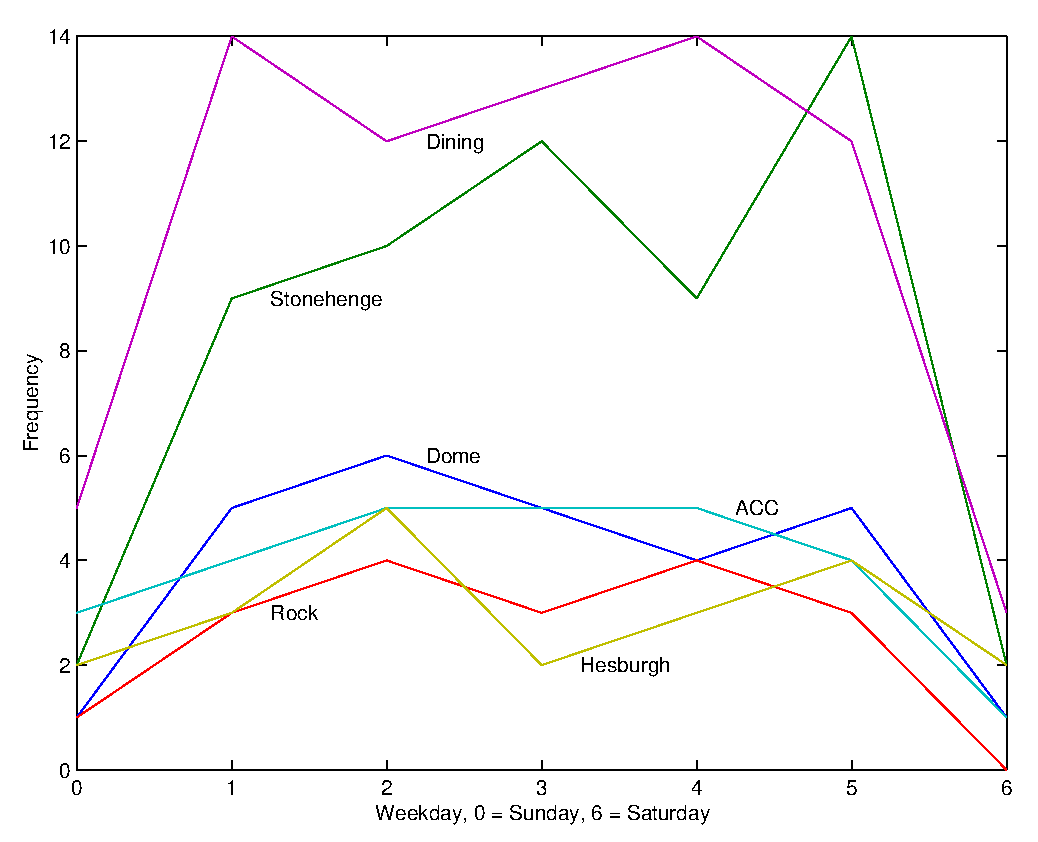
\includegraphics[scale=0.8]{sample_nd}}
    \caption{Location distributions by day of where, where the X axis
      is the weekday (0 through 6), and the Y axis is the sighting
      frequency}
    \label{fig:bogus3}
  \end{center}
\end{figure}

Gnus typically tend to come out when there are large gatherings of
humans with food.  Gnus work very hard at providing us with all the
things that we like (trees, dirt, air, etc.), and so we should freely
give them food.  They will come up and stand a respectful distance
away from you, waiting to see if they will be rewarded for their
efforts.  If you offer some food, they will take it and back off a
respectful distance in order to consume their food while leaving you
to your ``personal space.''  

\section{Groovin' Gnus}
\label{sec:groovin-gnus}

Gnus do tend to stay away from humans in their normal day-to-day
workings.  This is mainly because humans don't, for the most part,
understand what they are doing.  If a Gnu is working, and a human
approaches it, the Gnu will tend to drop whatever it is doing and run
away.  This is probably do to the tendency for humans to have ``group
meetings'' and ``productivity seminars.''  Most Gnus are deathly
afraid of such overmanagement, and run at the slightest hint of it,
for fear that it will cripple their real work.

It is interesting, however, that Gnus have chosen an Institution of
Higher Education for their BOO.\footnote{Base of Operations.}  It is
often said that:
\begin{quote}
  Academic politics are the dirtiest, meanest, ugliest, and generally
  the most low-down, in-your-face, and kick-em-while-they're-down than
  anywhere else (even Washington D.C.)  because the stakes are so low.
\end{quote}
It has been hypothesized that the Gnus are subtly trying to affect a
change for the better (i.e., eliminating the overmanagement problems)
by working the very system that they are trying to change, from
within.  That is, the graduates from Notre Dame can learn from the
examples of the Gnus here, and run screaming (or chattering) at the
slightest hint of overmanagement, and let the real work proceed
unhindered.

% % uncomment the following lines,
% if using chapter-wise bibliography
%
% \bibliographystyle{ndnatbib}
% \bibliography{example}



%
% Chapter 2
%

%
% Modified by Megan Patnott
% Last Change: Jan 18, 2013
%
%%%%%%%%%%%%%%%%%%%%%%%%%%%%%%%%%%%%%%%%%%%%%%%%%%%%%%%%%%%%%%%%%%%%%%%%
%
% Modified by Sameer Vijay
% Last Change: Wed Jul 27 2005 13:00 CEST
%
%%%%%%%%%%%%%%%%%%%%%%%%%%%%%%%%%%%%%%%%%%%%%%%%%%%%%%%%%%%%%%%%%%%%%%%%
%
% Sample Notre Dame Thesis/Dissertation
% Using Donald Peterson's ndthesis classfile
%
% Written by Jeff Squyres and Don Peterson
%
% Provided by the Information Technology Committee of
%   the Graduate Student Union
%   http://www.gsu.nd.edu/
%
% Nothing in this document is serious except the format.  :-)
%
% If you have any suggestions, comments, questions, please send e-mail
% to: ndthesis@gsu.nd.edu
%
%%%%%%%%%%%%%%%%%%%%%%%%%%%%%%%%%%%%%%%%%%%%%%%%%%%%%%%%%%%%%%%%%%%%%%%%

%
% Chapter 2
%

\chapter{Gnu Things are Good Things for all Graduate Students or so it Seems}
\label{chap:golfing}

\section{Gnu See, Gnu Do, Gnu Goes Golfing with Green Golf Genes and
  Gesticulates Grapes}

So why do gnus do what they do?  This is a perennial question that has
yet to be answered definitively by scientists.  Is their future
somehow tied inexplicably with that of humans?  Hard to say, but we do
feed them a lot.  It has even been theorized that rotundness is a
symbol of status or class within the Gnus; those who are more
productive (i.e., cute, furry, friendly) will be fed more than those
who are less so.  So the more rotund, the higher status one has in the
Gnu society.

One could extrapolate this to mean that there is a super-Gnu out there
somewhere; the biggest, rotundest Gnu that you've ever seen, probably
of epic proportions!  This would have to be the Leader of Gnus, or LoG
for short.  But the LoG would definitely have to be the cutest,
furriest, and most friendly Gnu that you've ever seen.

\subsection{The LoG}

So how does the LoG get chosen?  Ultimately by humans.  So we can say
that the Gnu society is perhaps the truest democracy that has ever
existed; the leader is chosen by merit, and chosen by complete
outsiders.  As such, the LoG must truly epitomize all that Gnus stand
for: opposedness to overmanagement, cuteness, friendliness, and
furriness~\citep{gloonson98:_gnuly_discov_gnus}.  The gnus themselves
vote at an anual election, based upon these attributes (campagaining
is an anethema to Gnus; see Section~\ref{sec:groovin-gnus}).

\subsubsection{Election Data}
\label{sec:data}

Table~\ref{tbl:votes} shows the latest electoral college voting by the
LoG for the year 2000.  Each Gnu is scored on a scale of one to ten on
the attributes described above.  The results shown in the table are
average scores in each category for all votes; the Gnu's final score
is shown in the final column.

%
% Be aware that page-spanning tables a Very Odd Creatures.  The
% "longtable" environment in LaTeX does some deep Voodoo to make
% everything work out properly.  One of its deep incantations is to
% make the table appear as though it is double spaced.  You can fix
% this by trailing each line with "\\[-6em]" instead of just "\\".
% When using longtable it is also important to compile your file
% more than once. But you're probably already doing this to get
% the internal references correct, anyway.
%

\begin{center}
  \begin{longtable}{lccccc}
    \caption{Electoral College Results for the \NoCaseChange{LoG} Election in the Year
2000\label{tbl:votes}\/}\\
        \toprule
        Candidate\footnote{note all names begin with G} & Anti-management & Cuteness & Friendliness & Furriness & Aggregate \\
        \midrule
\endfirsthead % Everything above goes at the top of the 1st page only
% As with the first header, we don't want obscene amounts of space for
% subsequent headings either, and eliminate an em of whitespace.
  \caption[]{{\em Continued}}\\
  \midrule
  Candidate & Anti-management & Cuteness & Friendliness & Furriness & Aggregate \\
  \midrule
\endhead % Everything above here (and below the \endfirsthead) goes at the top
         % of continuation pages.  The [] argument prevents a duplicate
         % entry from appearing in the table of contents.
% The following 3 lines are provided as an example only -- per ND
% guidelines, the footer at the bottom of a page for a longtable
% should not have a bottom line.  Only the absolute bottom of the
% table should have a final \bottomline

%  \midline
%  \multicolumn{6}{|r|}{\textit{continued}\ldots} \\
%  \bottomrule
\endfoot % The above section goes at the bottom of continuation pages
  \bottomrule
\endlastfoot % The very last bottom of the table
    Glen & 6.2 & 7.0 & 6.1 & 9.8 & 7.2 \\
    Goober & 6.9 & 2.1 & 5.7 & 4.1 & 4.6 \\
    Genevra & 2.2 & 2.0 & 1.1 & 1.1 & 1.6 \\
    Greg & 8.3 & 0.4 & 1.1 & 9.5 & 4.8 \\
    Gina & 6.0 & 7.8 & 6.4 & 4.9 & 6.2 \\
    Geof & 1.1 & 8.7 & 3.7 & 7.3 & 5.2 \\
    Grendel & 2.8 & 1.7 & 3.4 & 3.2 & 2.7 \\
    Geronimo & 1.2 & 1.2 & 8.8 & 2.2 & 3.3 \\
    Gabrielle & 4.7 & 3.6 & 0.8 & 2.0 & 2.7 \\
    Giovani & 8.4 & 5.8 & 3.4 & 7.4 & 6.2 \\
    Graham & 4.7 & 5.8 & 5.3 & 0 & 3.9 \\
    Gil & 5.9 & 4.0 & 5.5 & 7.6 & 5.7 \\
    Gerald & 2.0 & 3.7 & 8.0 & 4.3 & 4.5 \\
    Guilani & 7.7 & 3.9 & 2.7 & 6.4 & 5.1 \\
    Guido & 7.6 & 4.3 & 6.5 & 1.0 & 4.8 \\
    Godzilla & 5.1 & 2.2 & 5.3 & 6.9 & 4.8 \\
    Gail & 5.7 & 7.9 & 4.1 & 1.0 & 4.6 \\
    Garth & 4.7 & 7.1 & 2.5 & 3.0 & 4.3 \\
    Gavin & 1.1 & 9.5 & 0.4 & 8.0 & 4.7 \\
    George & 9.5 & 4.5 & 9.1 & 7.5 & 7.6 \\
    Gunnar & 1.4 & 5.8 & 4.8 & 6.2 & 4.5 \\
    Gillian & 7.6 & 9.0 & 6.4 & 4.6 & 6.9 \\
    Greta & 1.5 & 0.5 & 0.9 & 7.7 & 2.6 \\
    Gabby & 1.2 & 3.3 & 7.0 & 2.1 & 3.4 \\
    Gaetena & 6.8 & 1.9 & 4.1 & 8.3 & 5.2 \\
    Ganet & 2.3 & 1.1 & 8.5 & 7.3 & 4.8 \\
    Gardenia & 1.8 & 9.5 & 9.9 & 3.0 & 6.0 \\
    Genna & 5.2 & 3.7 & 3.4 & 3.8 & 4.0 \\
    Genesis & 1.7 & 8.3 & 6.7 & 4.9 & 5.4 \\
    Genaveve & 4.7 & 8.9 & 3.4 & 9.2 & 6.5 \\
    Gene & 3.3 & 6.9 & 0.6 & 5.5 & 4.0 \\
    Gilda & 5.2 & 4.6 & 9.9 & 1.4 & 5.2 \\
    Goldie & 8.9 & 9.1 & 2.0 & 8.2 & 7.0 \\
    Grace & 5.9 & 3.2 & 3.1 & 4.3 & 4.1 \\
    Gretchen & 4.5 & 6.5 & 1.6 & 1.3 & 3.4 \\
    Garrick & 4.8 & 5.7 & 9.4 & 5.1 & 6.2 \\
    Gallagher & 7.4 & 0.4 & 7.6 & 0.4 & 3.9 \\
    Gerry & 1.4 & 8.8 & 4.7 & 0.5 & 3.8 \\
    Gertrude & 9.1 & 8.3 & 0.4 & 5.5 & 5.8 \\
    Gehosephet & 6.6 & 2.9 & 8.3 & 4.4 & 5.5 \\
    Gohn & 8.7 & 2.6 & 7.4 & 2.3 & 5.2 \\
    Gibby & 8.7 & 6.9 & 4.7 & 7.2 & 6.9 \\
  \end{longtable}
\end{center}

As you can see from Table~\ref{tbl:votes}, George (my favorite Gnu)
won for the year 2000, with an aggregate score of 7.6.

% % uncomment the following lines,
% if using chapter-wise bibliography
%
% \bibliographystyle{ndnatbib}
% \bibliography{example}



%
% Appendix (optional)
%

\appendix

%
% Modified by Sameer Vijay
% Last Change: Wed Jul 27 2005 13:00 CEST
%
%%%%%%%%%%%%%%%%%%%%%%%%%%%%%%%%%%%%%%%%%%%%%%%%%%%%%%%%%%%%%%%%%%%%%%%%
%
% Sample Notre Dame Thesis/Dissertation
% Using Donald Peterson's ndthesis classfile
%
% Written by Jeff Squyres and Don Peterson
%
% Provided by the Information Technology Committee of
%   the Graduate Student Union
%   http://www.gsu.nd.edu/
%
% Nothing in this document is serious except the format.  :-)
%
% If you have any suggestions, comments, questions, please send e-mail
% to: ndthesis@gsu.nd.edu
%
%%%%%%%%%%%%%%%%%%%%%%%%%%%%%%%%%%%%%%%%%%%%%%%%%%%%%%%%%%%%%%%%%%%%%%%%

%%%%%%%%%%%%%%%%%%%%%%%%%%%%%%%%%%%%%%%%%%%%%%%%%%%%%%%%%%%%%%%%%%%%%%%%
%
% Appendix
%
%%%%%%%%%%%%%%%%%%%%%%%%%%%%%%%%%%%%%%%%%%%%%%%%%%%%%%%%%%%%%%%%%%%%%%%%

\chapter{GNU GENERALISMS}

\section{Definitions}

Several definitions are presented in Table~\ref{tbl:defs} to show both
how to do rotated, line-spanning tables, as well as to define some
commonly used Gnu terms.

\begin{landscape}
\begin{table}
\centering
\caption{Commonly used \NoCaseChange{Gnu} Terms \label{tbl:defs}}
\begin{tabular}{lp{5in}}
\toprule
Term & \multicolumn{1}{c}{Definition} \\
\midrule
Gnu & Small furry animal that is related to the squirrel 
(although they won't admit it). \\
LoG & Abbreviation for the ``Leader of Gnus''.  See
Chapter~\ref{chap:golfing}. \\
Twizzlers & Red, twisty candy that is among the most favorite of Gnu
foods.  Gnus frequently appear overly cute and friendly to humans
bearing twizzler packages.  This is known as ``trolling for twizzlers''
among the Gnus. \\
\bottomrule
\end{tabular}
\end{table}
\end{landscape}

Finally, Table~\ref{tbl:rotated-rankings} shows the top ten Gnus from
Table~\ref{tbl:votes} ranked in order by their aggregate score (along
with some of the raters' comments).  This follows a long-standing Gnu
tradition of self-improvement through public announcement of score
(which some associate with military
origins~\citep{galmira98:_gnus_milit}).  Indeed, this very table has
been observed in the Gnu lodge where it was posted for peer review
\citep{gairley2000}.


\begin{landscape}
% set the caption width to be somewhat short since our table is narrow
% Notice the special commands that we use here to get the right line in the
% table.  Using \hrule is *not* the Right Thing to do here -- use
% \cmidrule.  We use the LaTeX \newcommand simply for convenience.
%
% The longtable package does some nasty voodoo to make \hline work OK.
% So on with the goods
\setlength\LTcapwidth{4.5in}
\begin{longtable}{lcp{4.5in}}
% Note that after the caption line we remove 2em worth of space but in the
% longtable of Chapter 2 we only remove 1em.  This is because a normal 
% \toprule has no space above it, but here we are using cmidrule which does 
% have padding above which we must account for.
  \caption{Top Ten \NoCaseChange{Gnus} From
    Table~\NoCaseChange{\ref{tbl:votes}} With Reviewer Comments.
    \NoCaseChange{Gnus} are Listed Below in Alphabetic Order.
    \label{tbl:rotated-rankings} }\\
  \toprule
  Candidate & Aggregate score & \multicolumn{1}{c}{Reviewer Comments}\\
  \midrule
\endfirsthead
  \caption[]{{\em Continued}} \\  % Just like in Chp. 2
  \midrule
  Candidate & Aggregate score & \multicolumn{1}{c}{Reviewer Comments}\\
  \midrule
\endhead
\endfoot
  \bottomrule
\endlastfoot
George & 7.6 & George is an excellent candidate for the LoG.
  Slightly low C, but hopefully, this 7.6 will be high enough! \\
Glen & 7.2 & A little weak on AM and Fr, but good scores overall.  One
  or two more years of experience should be enough. \\
Goldie & 7.0 & Dismal score in Fr; suspect it had something to do with
  strenuous weight loss program this past year. \\
Gillian & 6.9 & Excellent C, but a little shabby on the Fu.  Suggest
  more roughage. \\
Gibby & 6.9 & Reasonable scores, but need to work on Fr.  Gibby is
  definitely not a morning Gnu. \\ 
Genaveve & 6.5 & Very low Fr; perhaps more coffee?  Suggest practicing
  ``cute faces'' in the mirror several hours per day.  \\
Giovani & 6.2 & Very low Fr; suspect hanging out with Genaveve too
  much. \\
Gina & 6.2 & Mediochre Fu, somewhat low AM.  Perhaps a future in
  marketing or advertising? \\
Garrick & 6.2 & Fairly low AM.  Fu could be better as well; buy a
  comb.  And a mirror.  Immediately.  \\
Gardenia & 6.0 & Dismal AM; very low Fu.  Seems to care more about
  meeting agendas than personal appearance. \\
\end{longtable}
\end{landscape}


% % uncomment the following lines,
% if using chapter-wise bibliography
%
% \bibliographystyle{ndnatbib}
% \bibliography{example}



%
% Back stuff
%

% % comment out the following three lines
% if using chapter-wise bibliography

 \backmatter
 \bibliographystyle{abbrvnat} % The standard abbrvnat style should be acceptable. Also provided with both the advanced and standard
 \bibliography{example}       % distributions are nddiss2e and nddiss2enoarticletitles style options.
% If you prefer to manually enter your bibliography, that is fine. Comment out the previous two lines, and enter your bibliography
% as usual. Note that if you choose this route, formatting the bibliography is your responsibility. An example is below, including the
% optional arguments necessary for author-date style citations.
%	\begin{thebibliography}{9}
%		\bibitem[Galmira(1998)]{galmira98:_gnus_milit} G.\ Galmira. Gnus and the military -- a secret conspiracy? \emph{Growing Towards Gnu}, III(7):22--183, September 1998.
%		
%		\bibitem[Ganston and Greenfield(1998)]{gnus98:_gerry_ganst} G.\ Ganston and G.\ Greenfield. \emph{Gnus and You: The Art of Being New}. volume I. Grapping Books, NY, August, 1998.
%		
%		\bibitem[Gloonston(1998)]{gloonston98:_gnuly_discov_gnus} G.\ Gloonston. Newly discovered gnus: The LoG. \emph{Growing Towards Gnu}, II(12):23---57, March 1998.
%		
%		\bibitem[Greenfield(1996)]{greenfield96:_gettin_know_gnu} G.\ Greenfield. \emph{Getting to Know Gnu}. PhD thesis, Geoffrey Garfield School of Gnus, August 1996.
%		
%		\bibitem[van Gairley(2000)]{gairley2000} G.\ van Gairley. Gnu's review. Website, 2000. \url{http://www.gairley.gnu}.
%	\end{thebibliography}

\end{document}

% End of ``example.tex''
